\documentclass[conference]{IEEEtran}
\IEEEoverridecommandlockouts
% The preceding line is only needed to identify funding in the first footnote. If that is unneeded, please comment it out.
\usepackage{cite}
\usepackage{amsmath,amssymb,amsfonts}
\usepackage{algorithmic}
\usepackage{graphicx}
\usepackage{textcomp}
\def\BibTeX{{\rm B\kern-.05em{\sc i\kern-.025em b}\kern-.08em
    T\kern-.1667em\lower.7ex\hbox{E}\kern-.125emX}}
\begin{document}

\title{Beating uncertainty in racing bot evolution through enhanced
  exploration and pole position selection}

\author{\IEEEauthorblockN{Mohammed Salem\IEEEauthorrefmark{1},
Antonio M. Mora\IEEEauthorrefmark{2} and
Juan J. Merelo\IEEEauthorrefmark{3}}

\IEEEauthorblockA{\IEEEauthorrefmark{1}Dept. of Computer Sciences, University of Mascara, Algeria. \\Email: salem@univ-mascara.dz}
\IEEEauthorblockA{\IEEEauthorrefmark{2}Dept. of Signal Theory, Telematics and Communications, ETSIIT-CITIC, University of Granada, Spain. \\Email: amorag@ugr.es}
\IEEEauthorblockA{\IEEEauthorrefmark{3}Dept. of Computer Architecture and Computer Technology. University of Granada, Spain. \\Email: jmerelo@geneura.ugr.es}
}

\maketitle

\begin{abstract}

One of the main problems in the design through optimization of car
racing bots is the inherent noise in the optimization process: besides
the fact that the fitness is a heuristic based on what we think are
the keys to success and as such just a surrogate for the ultimate
objective, winning races, fitness itself is uncertain due to the
stochastic behavior of racing conditions and the rest of the
(simulated) racers. The  fuzzy-based genetic controller for the car
racing simulator TORCS we have defined in previous works is based on two fuzzy sub-controllers, one for deciding on the wheel steering angle and
another to set the car target speed at the next simulation tick. They
are both optimized by means of an Evolutionary Algorithm, which
considers an already tested fitness function focused on the
maximization of the average speed during the race and the minimization
of the car damage. The noisy environment asks for keeping diversity
high during evolution, that is why we have added a Blend Crossover (BLX-$\alpha$) operator, which is, besides, able to exploit current results at the same time it explores. Additionally, we try to address uncertainty in
selection by introducing a novel selection policy of parents based in races, where the individuals are grouped and compete against others in several races, so the first 5 will remain in the population as parents.
Several experiments have been conducted, testing the value of the
different controllers. The results show that the combination of a
dynamic BLX-$\alpha$ crossover operator plus the \textit{pole position selection} policy clearly beats the rest of approaches. Moreover, in the
comparison of this controller with one of the participants of the
prestigious international Simulated Car Racing Championship, our
autonomous driver obtains much better results than the opponent.

\end{abstract}
\begin{IEEEkeywords}
Videogames, Simulated Car Racing, TORCS, Fuzzy Controllers, Autonomous Drivers, Genetic Algorithms, BLX-$\alpha$ Crossover, Optimization, Race-based Selection, Uncertainty
\end{IEEEkeywords}

%%%%%%%%%%%%%%%%%%%%%%%%%%%%%%%   INTRODUCTION   %%%%%%%%%%%%%%%%%%%%%%%%%%%%%%%
%
\section{Introduction}
\label{sec:intro}

% >>>>>> TODO: Rewrite Introduction -> JJ  <<<<<<<<<<<<<
% NEW SELLING POINTS: 
% 	- Tried selection based in races every 5 generations (in addition to at the end)
%	- Implemented BLX-Alpha Crossover to enhance results
%	- Tested against a "real" controller which finished in the
%	middle of classification at the last Car Racing Competition
%	(in 2009, but anyway it has not been improved and it's the
%	only one we have)
% The introduction is then the same one as before? - JJ

Games are, in many cases, closes and controlled environments, mini or
simulated worlds that allow you to test techniques that will then
eventually be applied in real life, probably combined with other
different technologies to tackle its complexity and variability. Car
racing simulation includes many of the factors that are present in
autonomous driving: tracks are very different and not known in
advance, there are other vehicles present on the track, and the
conditions change according to weather, and car deteriorates with
damage. Car is also aware of this only through a set of limited
sensors, and it will have to take a decision on
speed and steering that is optimal in several different
senses \cite{Autodriv2006}, including, depending on the context, the
possibility of beating a set of opponents in a simulated race.


Since testing different autonomous driving methodologies in real life is
usually reserved to just a few big players, methodologies 
as well as algorithms are usually tested in simulated environments;
these simulated environments, at the same time, offer the incentive of
competition among your system and others. In this paper, we will be
using The Open Racing Car Simulator (TORCS) \cite{torcs4}, a very
realistic racing simulator which offers a great testbed for the
implementation and evaluation of autonomous drivers.  
It has been used several times for the celebration of Artificial
Intelligence (AI) competitions, where the aim is to create the best
autonomous driver for racing
\cite{SimulatedCarRacing-2008,SimulatedCarRacing-2010,Torcs3,manualTORCS}. Besides being able to test your car against other cars that have been published, it can be used as a standalone environment to optimize driving in a
solo race. 

Evolutionary Algorithms (EAs) \cite{EAs_Back96} have been frequently
applied as a general-purpose optimization method in this area,
generally combined with behavioural engines that rule different parts
of the car
\cite{Floreano2004,CarRacing_Pelta09,SAES2012,torcs2012}. These
driving engines have included lately fuzzy controllers
\cite{Guadarrama2008, LFAG, PerezEvolvingFuzzy09}. These controllers
use fuzzy Logic \cite{Fuzzy2011}, a  technique that is quite suitable
for defining this kind of autonomous agents, since they are in part
inspired by the human reasoning when driving. A fuzzy controller works
with linguistic variables, and will for instance turn {\em slightly}
to the right when the next curve is {\em close}, but these controllers
have to be designed to map properly inputs to desired outputs in
particular situations. 

From the point of view of optimization, one of the main problems is
that the environment is always going to change; this is correctly
reflected in the simulators used, and it means that the score (and
thus the ranking, if that's the eventual target) will always change,
making selection of the {\em best} or {\em winning} controller
probabilistic at best. This uncertainty is a challenge from two points
of view: non optimal (non-winning) controllers might be selected just
by chance, since they were assigned a score favored by that
uncertainty, and, once they are selected, that might make the
algorithm explore zones around some controllers that have been
selected just by chance, and leave others unexplored. For these two
reasons, there are two challenges that we intend to approach in this
paper: reduce uncertainty in selection of the ``best'', and keep
diversity high to not exploit just the areas around those individuals
whose score might have been favored by chance at a certain point in
the evolution process.

% Antonio - Previous works
Previously, the authors presented an approach
combining two specialized fuzzy controllers, designed by hand, that
were able to decide the car's proper steering angle and desired speed
at every single point (or tick) during a race \cite{salem_evo17}. This
driver was later improved \cite{salem_evo18} optimizing the parameters of
their membership functions by means of a Genetic Algorithm
\cite{GAs_Goldberg89}; this automated design improved manual one
obtaining several controllers that were able to beat the initial
hand-designed controller in a race, as well as other published
controllers. Finally, the authors enhanced the controller in the last paper \cite{salem_cig2018} by means of the definition of new fitness functions. The selection of the best controller at the end of the evolution was based on a set of races among the best 4 solutions, getting a better driver than in previous studies.

This proved that evolutionary algorithms were able to get the fuzzy
controller parameters better than a hand-made design, but at the same
time revealed several challenges. In general, evolutionary algorithms
optimize the fitness function that is used; evolved fuzzy controllers
(hereafter FCs) will be eventually as good as the fitness function allows. 
But in this particular case we cannot use as fitness function the position
obtained by the FC in every possible race on every possible track with
every possible opponent, so we have to settle for a {\em surrogate} of
the fitness in a very limited environment. First we opted for
eliminating opponents and making evaluations in solo races; then we
chose a particular track that combined straight segments as well as
some curves and did not take too long to run, and eventually we had to
decide what factors related to speed, damage and lap time were going
to be effectively included in the final fitness function. 

Results were encouraging, but it is still a surrogate model. As such a
model, we need to decide on the best track to perform {\em training}
and also the solo race measures with the biggest impact in the
eventual racing performance. This is why in this paper we have
combined into the fitness function only those terms related with speed
during race (to maximize) and damage (to minimize) - the most
important factors - in two different approaches. 
Besides, the fitness evaluation process has a certain amount of uncertainty because damages and some track conditions can randomly vary in different
evaluations. This is why instead of selecting directly the driver as
we did before, we will be using an actual race among the best drivers
to select the best one.

The two new techniques introduced in this paper, namely, ``Pole''
selection and BLX-$\alpha$ crossover, try to improve on previous
results by first relying less on the surrogacy of the fitness function
to select the best individuals. The Pole selection will use fitness to
select a few individuals that will race against each other; racing
will {\em smooth out} randomness in the fitness by putting them in a
more real environment; racing cars against each other will offer a
result that varies much less than simply comparing fitness. But, even
so, uncertainty is present in the fitness and we should avoid
excessive exploitation of the results. The BLX-$\alpha$ crossover we
have introduced takes care of this aspect.

The rest of the paper is organized as follows. Next we present the
state of the art, to be followed by a description of the TORCS
simulator \ref{sec:torcs}, the defined fuzzy controllers \ref{sec:subcontrollers} and a deep explanation of the Genetic Algorithm implemented and tested in this work in Section \ref{sec:GA_optimization}. 
%Then, in Section \ref{sec:new-opponent}, we briefly introduce a real controller which participated in previous editions of the Simulated Car Racing Competition and which will be considered as a new opponent for comparisons.
After it, the experiments conducted and the obtained results are described in Section \ref{sec:results}. Finally, conclusions and future lines of work will be presented in section \ref{sec:conclusions}.


%%%%%%%%%%%%%%%%%%%%%%%%%%%%%%  STATE OF THE ART  %%%%%%%%%%%%%%%%%%%%%%%%%%%%%%
\section{State of the Art}
\label{sec:soa}

% This is almost the same as the last one, if not exactly the same. We
% should really change it more than introduction or other things. - JJ
TORCS has become one of the
main environments for research on AI since its launch in 2007
\cite{torcs4}. {\em Autonomous} cars, or {\em bots}, created to win
races in this environment need to set the optimal parameters for the
cars \cite{Kole-ParamCarTunning12} with the ultimate objective of
participating in one of the Simulated Racing Car Competitions
\cite{SimulatedCarRacing-2008,SimulatedCarRacing-2010}. However, the
problem of racing a car itself is a challenge, and thus it has been used as a subject
of research from the beginning even without the intention of
participating in the competition; in any case, published controllers
are always used as the state of the art reference, and any new bot
should be compared against at least those that are available.

% This should be much more systematic. It should say:
% These are the kind of controllers there are; these are the kind of
% techniques that are used, these are the results obtained
There are many possible ways of approaching the design of an automatic
driver for a car, and through the use of different simulators and
techniques, they have probably been pursued in one way or the
other. In a nutshell, you have to provide for a way to drive the car,
in real time, from the inputs gathered by the car. TORCS offer a rich
array of sensors, but it also includes vision  \cite{Floreano2004}, although most papers do
rely only on the sensors, since they offer enough information for
driving the car.

The way sensors and effectors are connected also varies. The simulator
itself offers a baseline controller, but that is also configurable and
you can choose to wire it in some other way
\cite{cussat2016dangerousness}. While this might be effective for some
specific purposes like the one used in the paper, evaluate the
dangerousness of the track, in general working with an already wired
controller that is able, for instance, to work towards a target speed
instead of dealing directly with throttle and braking is much more
convenient. This default controller, as a matter of fact, lets you
choose what you actually want to change or optimize. Some people opt
for changing just the steering \cite{CarRacing_Pelta09,

Our own work tried to take the state of the art further by introducing
a fuzzy controller evolved via evolutionary algorithms in
\cite{salem_evo17}, which evolved a fuzzy-based driver considering the
target speed in addition to controlling steering (two fuzzy
sub-controllers). 
This controller was also enhanced in a further work \cite{salem_evo18}
optimizing the parameters of the membership functions by means of a
real coded genetic algorithm, obtaining a noticeable improvement in
performance. Lately, we presented \cite{salem_cig2018} an improvement on our proposal considering parameter-less fitness functions and a final selection of the best based in additional races involving the top 4 individuals and other rivals.

In this study we build on this last approach, focusing on the best
fitness function to date and the final selection process, but also
involving two new mechanisms during the evolution: a \textit{Blend
  Crossover operator} to control the balance between exploration and
exploitation, and a \textit{Race-based selection of parents}, aiming
to choose real good drivers in races, rather than just select those
with the highest fitness values, in order to avoid somehow the
uncertainty/noise present on the problem
\cite{merelo2016statistical}. 


%%%%%%%%%%%%%%%%%%%%%%%%%%%%%%  TORCS  %%%%%%%%%%%%%%%%%%%%%%%%%%%%%%

\section{The Open Racing Car Simulator}
\label{sec:torcs}

The framework in which this study has been conducted is TORCS \cite{torcs4}. It is an open source, multi-player, modular and portable racing simulator that allows users to compete against other computer-controlled opponents.
Its high degree of modularity and portability, together with the
realistic and real-time driving simulation, make it an ideal testbed
for artificial intelligence research, as stated in previous section.

Every car in TORCS includes  a large set of sensors \cite{Torcs3},
whose values the car can use during a race, such as distances to track borders, to rivals, current fuel, current gear, position in the race, speed, or damage, among others. See Figure \ref{fig:torcs-sensors}.

\begin{figure}[!ht] 
	\begin{center}
		\includegraphics[scale=0.35]{fig/torcs-sensors}
		\caption {TORCS capture showing some of the sensors that the car includes.}
		\label{fig:torcs-sensors}
	\end{center}
% Antonio - if we need space we can remove this image
\end{figure}


The sensor values are considered by any TORCS autonomous driver, or
{\em controller}, to manage the car using actuators \cite{Torcs3}: the
steering wheel, the accelerator, the brake pedal and the gearbox.   


%*****************************  FUZZY CONTROLLER  ******************************

\section{Fuzzy sub-controllers}
\label{sec:subcontrollers}

We initially proposed a controller \cite{salem_evo17} with the same modular architecture as the simple TORCS driver; however, the target speed and
steering angle are computed by means of two modular and specialized
fuzzy sub-controllers, which consider five position sensors. This is
the controller which will be improved by means of a GA in this
work.

The \textbf{fuzzy target speed sub-controller} aims to estimate the
optimal target speed of the car, both in straight parts and curves of
the track, taking into account two criteria: move as fast as possible
and be safe. This estimation is based on two general cases: if the car
is in a straight line, the target speed will take a maximum value
(\textit{maxSpeed} km/h). However, if it is close to a curve, the
controller will decrease the current speed to a value included in the
interval \textit{[minSpeed, maxSpeed]} km/h. 

This fuzzy controller has an output, the speed, and three input values (See Figure \ref{fig:torcs-sensors}):
\begin{itemize}
	\item Front = Track\_9: front distance to the track border (angle 0\textdegree).  
	\item M5 = max (Track\_8, Track\_10): max distance to the track border in an angle of +5\textdegree and -5\textdegree with respect to Front.
	\item M10 = max (Track\_7, Track\_11): max distance to track border in an angle of +10\textdegree and -10\textdegree.
\end{itemize}

It is a Mamdani-based fuzzy system \cite{iancu2012} with three
trapezoidal Membership Functions (MF) for every input variable. 
%The description of these fuzzy inputs and output are represented in Table
%\ref{tab:flouevar}. 
In \cite{salem_evo18} the different sets of parameters which define the membership functions were improved using a Genetic Algorithm to obtain the best results.

Moreover, the controller is based in a set of fuzzy rules, designed to
maximize the car speed depending on the distance to the track
border. These rules can be consulted in \cite{salem_evo17}.
% Antonio - TODO: Include the rules if there is available space?
%
%The fuzzy rules are:
%
% \begin{itemize}
% {\small
% 	\item \texttt{IF Front is High THEN TargetSpeed is TS1}
% 	\item \texttt{IF Front is Medium THEN TargetSpeed is TS2}
% 	\item \texttt{IF Front is Low and M5 is High THEN TargetSpeed is TS3}
% 	\item \texttt{IF Front is Low and M5 is Medium THEN TargetSpeed is TS4}
% 	\item \texttt{IF Front is Low and M5 is Low and M10 is High THEN TargetSpeed is TS5}
% 	\item \texttt{IF Front is Low and M5 is Low and M10 is Medium THEN TargetSpeed is TS6}
% 	\item \texttt{IF Front is Low and M5 is Low and M10 is Low THEN TargetSpeed is TS7}\\
% }
%
% In addition, a crisp rule is added to obtain a maximum value of the target speed when the three input variables are as big as possible:\\
% {\small	
% \item \texttt{IF Front = MAXDISTSPEED or M5 = MAXDISTSPEED or M10 = MAXDISTSPEED THEN TargetSpeed = MAXSPEED}
% }
% \end{itemize}
%
% MAXDISTSPEED is the longest possible value for the track sensors, and MAXSPEED is the maximal speed for the specific car. 
% The output value is encoded by seven singletons TS1 to TS7, being respectively: 280, 240, 220, 180, 120, 60 and 30.\\
%
%
% %***********************************************
% \noindent
% \textbf{Fuzzy steering control sub-controller}\\
% %
%
The second is the \textbf{fuzzy steering sub-controller}, which aims to define the steer angle estimating and determining the target position of the car. 
%
The structure of this sub-controller is similar to the speed one, but it has the steering as output. Thus, the set of sensors considered is the same as in the speed case.

Then, as general rules: if the car is in a straight line, it will set as target position half width of the race track (central position of the lane). Whereas, if the car is near a right curve, it will approach the path leading to the right, with a space between the car and the border of the track to avoid the loss of control. The same approach is considered if the car is near a left curve.

In order to detect the curves, the controller focuses on the sensor values (M10, M5, and Front). So, if the value on Front sensor is the longest, there is a straight road; whereas if the values of M5 and M10 with positive angles (+5 and +10) are the longest, there is right curve; and the other way round.

It uses a base of rules which has been defined trying to model the behavior of a human driver \cite{salem_evo17}.

%, so, for this controller:
% Antonio - TODO: Include the rules if there is available space?

% {\small
% \begin{itemize}		
% 	\item \texttt{IF Front is High THEN steer is S1}
% 	\item \texttt{IF Front is Medium AND M10 is High THEN  steer is S2}
% 	\item \texttt{IF Front is Medium AND M10 is Medium AND M5 is Medium THEN steer is S2}
% 	\item \texttt{IF Front is Medium AND M10 is Medium AND M5 is Low THEN steer is S3}
% 	\item \texttt{IF Front is Low AND M10 is High THEN steer is S3}
% 	\item \texttt{IF Front is Low AND M10 is Medium AND M5 is Medium THEN steer is S4}
% 	\item \texttt{IF Front is Low AND M10 is Medium AND M5 is Low THEN steer is S4}
% \end{itemize}	
% }

% The values for S1 to S4 are respectively: 0, 0.25, 0.5, and 1.
% When M10=Track[7] we will take negative values of the steer (steer=-steer).

% These controllers were defined with our own criteria, but they could be far from being optimal, so, in the following section we apply a Genetic Algorithm for their improvement.


As stated, the designed fuzzy controllers have trapezoidal membership functions given by Equation \ref{eq:trapmf}.
In such a controller, fuzzy rules are applied to linguistic
terms. These terms, which qualify a linguistic variable, are defined
through membership functions, which, in turn, depend on a set of
parameters that `describes' their shape (and operation). Using a GA we
will optimize the parameters of the membership functions that
constitute the fuzzy partition of the linguistic variable
\cite{ThangG08}. The input linguistic variables in our problem,
\textit{Front, Max5} and \textit{Max10}, are represented by three
trapezoidal membership functions. 

A trapezoidal membership function in a finite universe of discourse \textit{[a, b]} can be defined by:

\begin{equation}
\mu_{A}(x)= \left \{
\begin{array}{ll}
\frac{x - x_{1}}{x_{2} - x_{1}},& x_{1} \leq x \leq x_{2}\\
1 , &x_{2} \leq x \leq x_{3}\\
\frac{x_{4} - x}{x_{4} - x_{3}},& x_{3} \leq x \leq x_{4}\\
0        ,& else\\	
\end{array}
\right.
\label{eq:trapmf}
\end{equation}
with:
\begin{equation}
x_{1} \leq x_{2} \leq x_{3} \leq x_{4}
\end{equation}
This MF function is defined by four parameters $x_{1}$, $x_{2}$,
$x_{3}$ and $x_{4}$ taking their values in the interval \textit{[a,
  b]}.% (See Figure \ref{fig:trapeze}).

\begin{figure}[!ht] 
	\begin{center}
		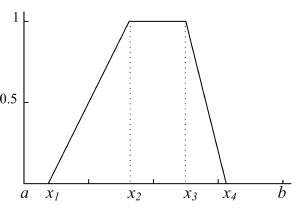
\includegraphics[scale=0.5]{fig/trapese}
		\caption {Trapezoidal MFs}
		\label{fig:trapeze}
	\end{center}
% Mohammed: Could we remove this figure?
% Antonio - if we need space, yes, otherwise, it does not matter I think
\end{figure}
And a fuzzy partition with \textit{n} trapezoidal membership functions
is defined by \textit{2n} variables (\textit{a =} $ x_{1}$,$x_{2}
$,. .., $x_{2n} $ \textit {= b})(Equation \ref{eq:e1}). In this case,
the representation is given by the
figure \ref{fig:at} 
\begin{figure}[!ht] 
	\begin{center}
		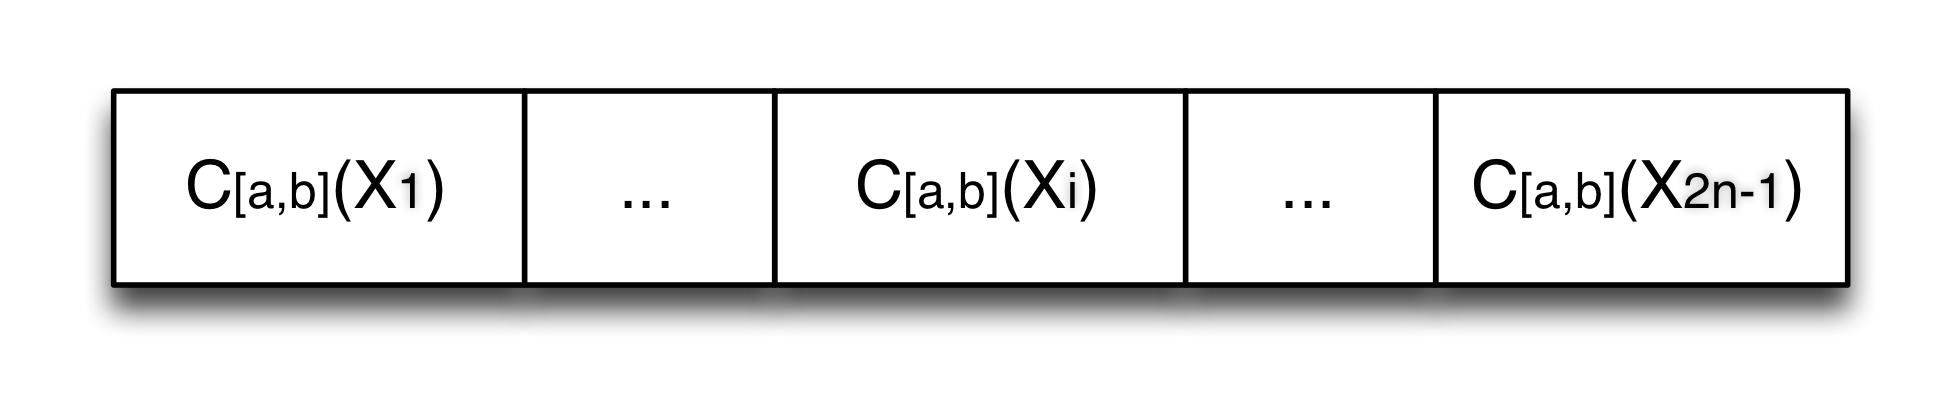
\includegraphics[scale=0.4]{fig/trapezoidal.png}
		\caption {Trapezoidal-shaped MFs coding}
		\label{fig:at}
	\end{center}
\end{figure}
with:
\begin{equation}
a = x_{1} \leq x_{2} \leq...\leq x_{2n-1} \leq x_{2n}=b 	
\end{equation}		

\begin{equation} 
\begin{tabular}{l}
$\mu_{A1}(x)=  \left \{
\begin{array}{ll}
1, &x_{1} \leq x \leq x_{2}\\
\frac{x_{3} - x}{x_{3} - x_{2}}, &x_{2} \leq x \leq x_{3}\\
0        , &x > x_{3}\\
\end{array} 
\right.$		\\ 	
$\mu_{Ai}(x)= \left \{
\begin{array}{ll} 
0, &x \leq x_{2i-2}\\
\frac{x - x_{2i-2}}{x_{2i-1} - x_{2i-2}}, &x_{2i-2} \leq x \leq x_{2i-1},n=2,...,i-1\\
1, & x_{2i-1} \leq x \leq x_{2i}\\
\frac{x_{2i+1} - x}{x_{2i+1} - x_{2i}},& x_{2i} \leq x \leq x_{2i+1}\\
0  , &x > x_{2i+1}\\
\end{array}  
\right.	$		\\
$\mu_{An}(x)= \left \{
\begin{array}{ll} 
0, &x \leq x_{2n-2}\\
\frac{x - x_{2n-2}}{x_{2n-1} - x_{2n-2}},& x_{2n-2} \leq x \leq x_{2n-1}\\
1 ,& x > x_{2n-1} 
\end{array} 
\right.$\\
\label{eq:e1}
\end{tabular}
\end{equation}

This is the base of the optimization conducted by the Genetic Algorithm, as it is described in the following section.


%%%%%%%%%%%%%%%%%%%%%%%%%%%%  OPTIMISING WITH GAS  %%%%%%%%%%%%%%%%%%%%%%%%%%%%

\section{Genetic Algorithm}
\label{sec:GA_optimization}

We proposed an optimization approach based in Genetic Algorithms (GAs) \cite{GAs_Goldberg89} aiming to find the optimal parameters of the membership functions of the two sub-controllers previously introduced. 

Thus, every individual is a vector of 18 values/parameters, 6 per variable. Figure \ref {fig:cromosome} illustrates the structure of the chromosome.
\begin{figure*}[!ht]	
  \begin{center}
    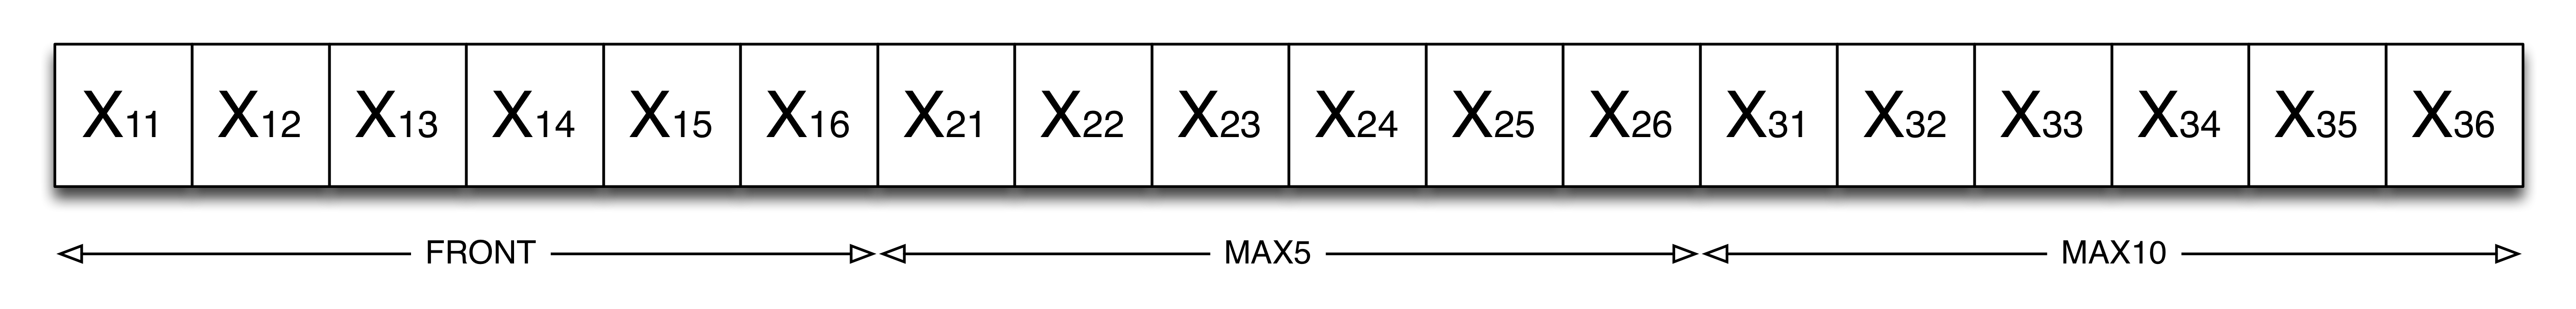
\includegraphics[width=12cm]{fig/chromosome2.png}
    \caption{Chromosome description}
    \label{fig:cromosome}	
  \end{center}	
\end{figure*}

The initialization of the chromosomes (first population) is performed by assigning random values inside a range of variation ($[0,100]$)
\cite{GAs_Goldberg89}, in order to start from feasible values
\cite{salem_evo17}. Since our work requires some precision and the variation interval of each parameter is not well known, we have considered a real coding
implementation \cite{elsayed13} in a vector that includes all variables to optimize.

The overall process is summarized in Figure \ref{fig:ga}. As it can be seen, TORCS is used during the evaluation step of every individual in the evolutionary process.

\begin{figure}[!ht]
  \label{fig:ga}
  \begin{center}
    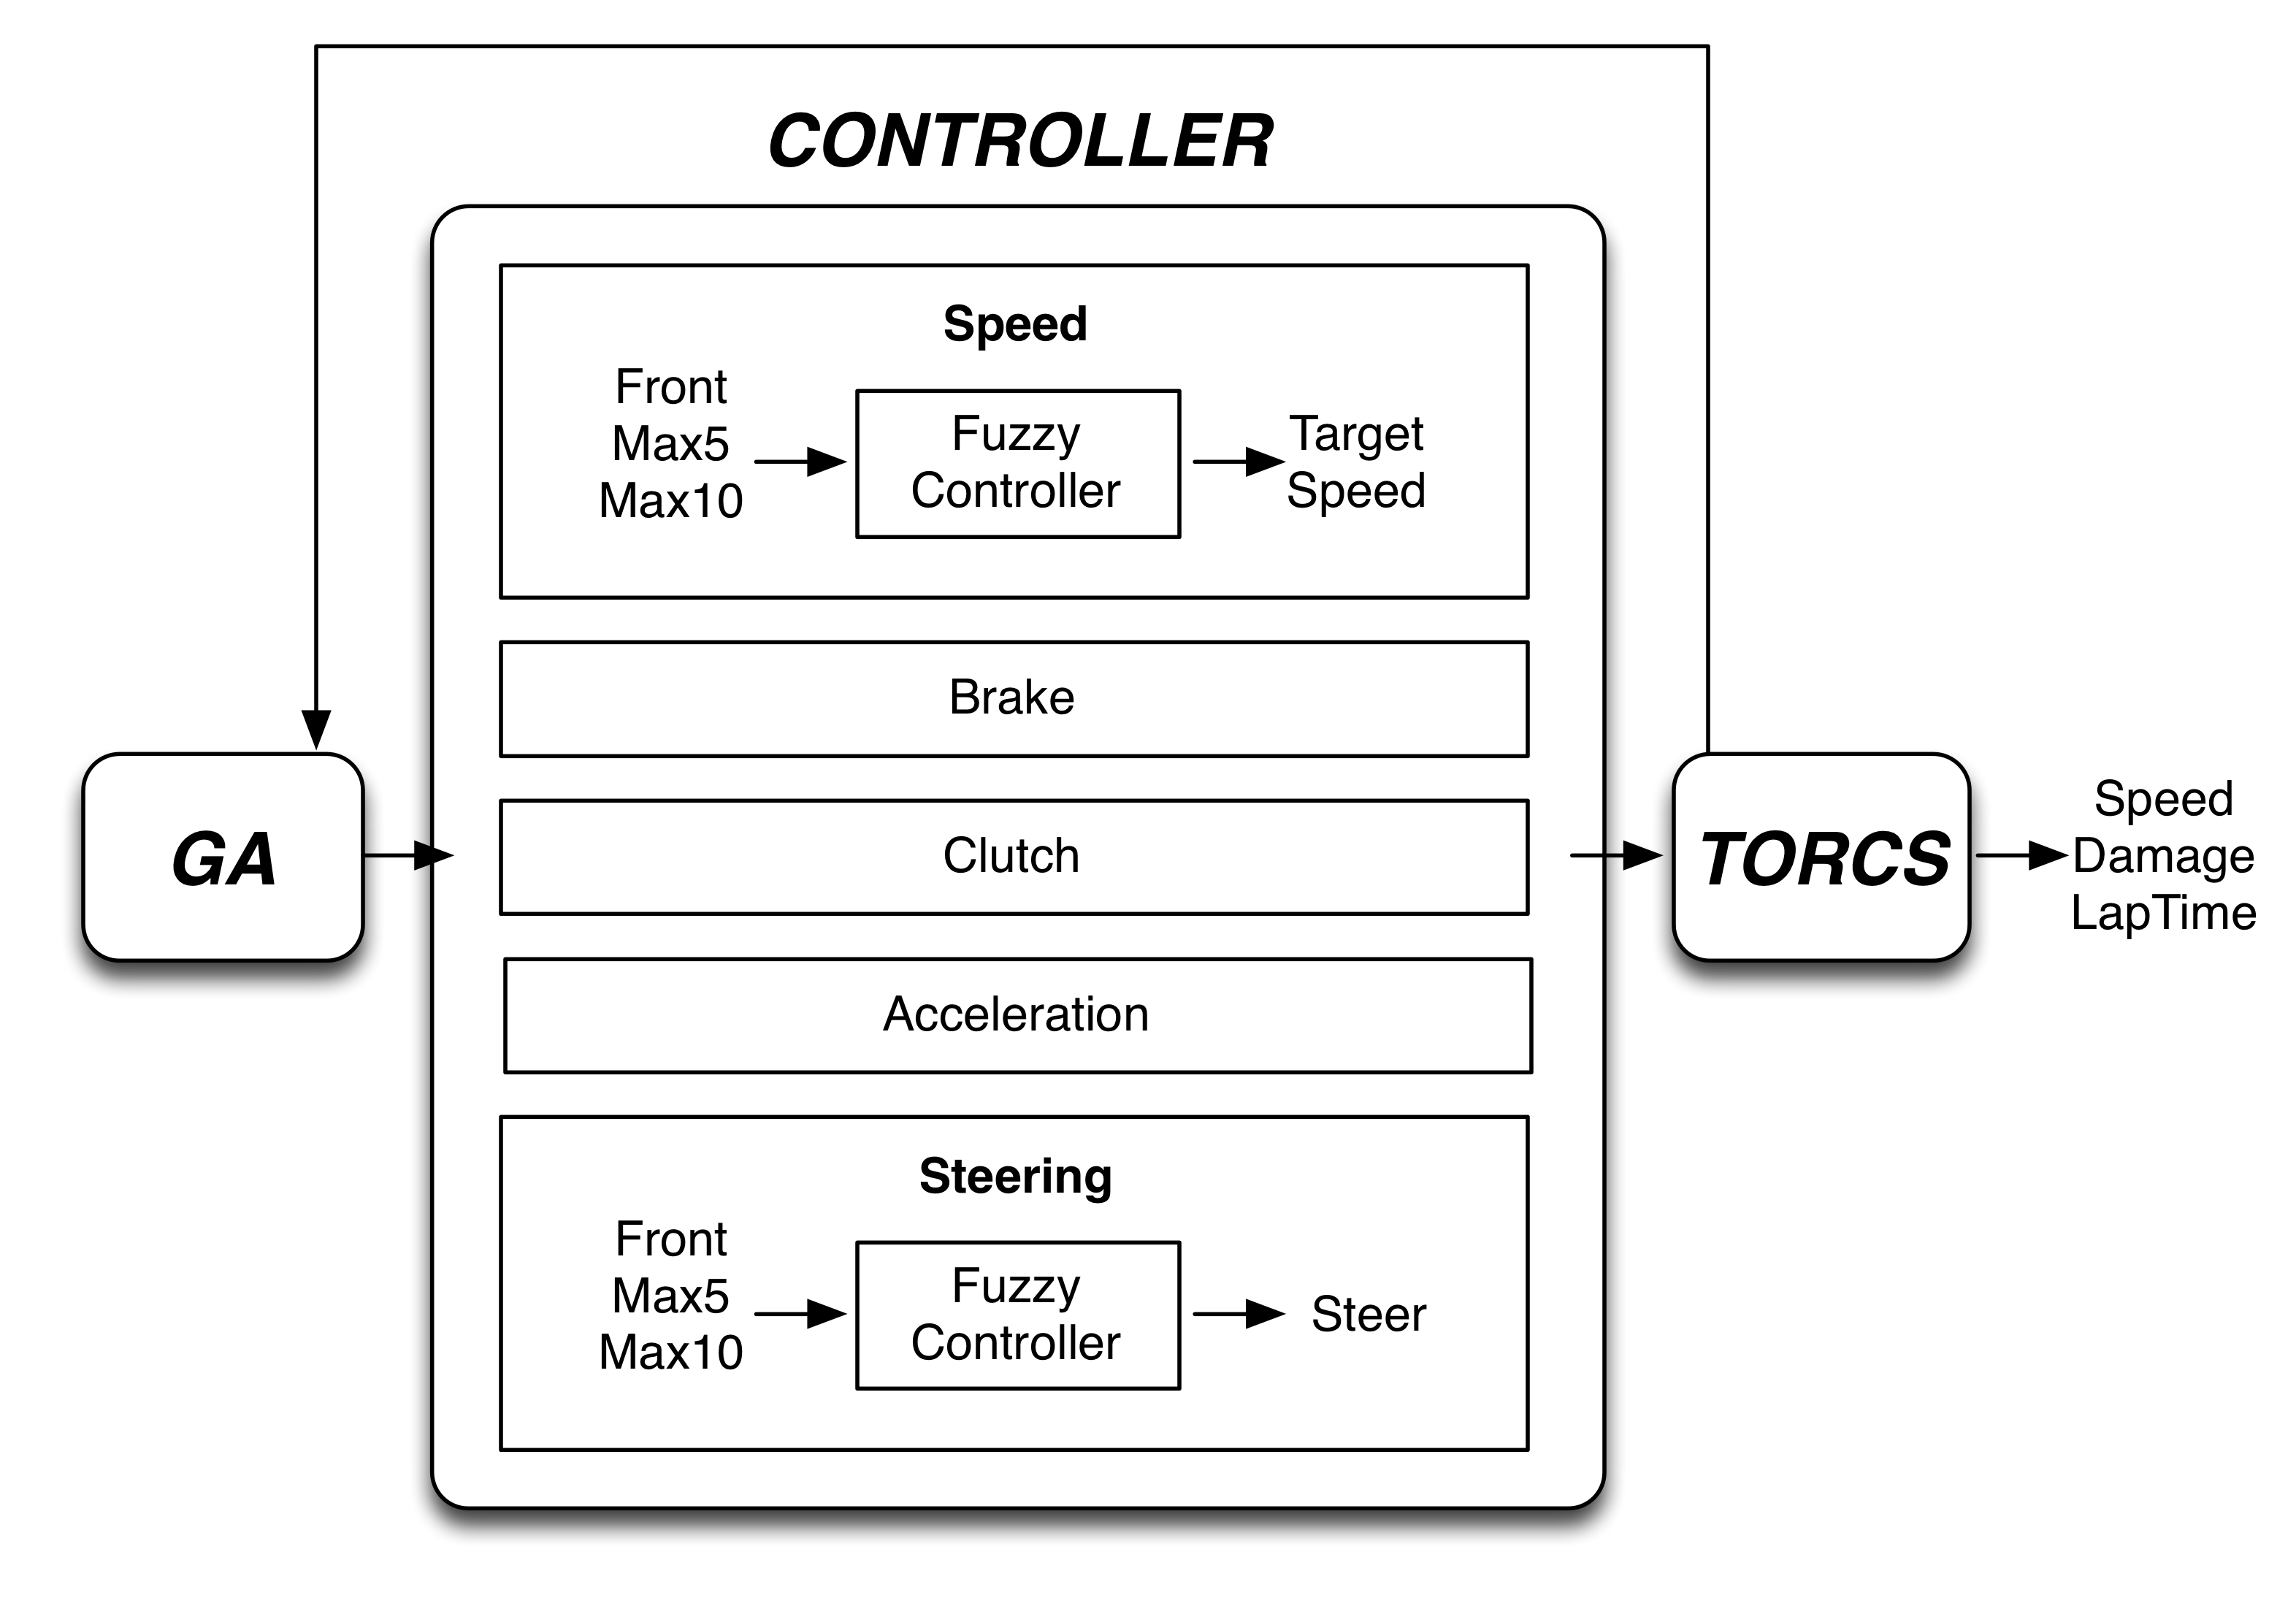
\includegraphics[width=9cm]{fig/flowchart}
  \end{center}
  \caption{Flowchart of  the optimization process of a TORCS fuzzy controller. To evaluate an individual we put the parameter values of the two sub-controllers in the corresponding chromosome, then we launch a race in TORCS with this configuration, obtaining the resulting values of Damage, Top Speed and Mean Lap Time. Individual's fitness value is computed using these values.}
\end{figure}

The evaluation of the individuals is based in different fitness functions, which we have tested in previous works \cite{salem_evo18}. In this study we will consider the one which yielded the best results in our previous paper \cite{salem_cig2018}, namely:

\begin{equation} \label{fit2}
	\begin{array}{lll}
	f_{AVS}= \frac{AVG(Speed)}{Damage+1}
	\end{array}
\end{equation}	

It is a parameter-less approach (no weights in the terms) \cite{Harik-ParameterLess99}, which is also more focused on the real objectives for a driver during a race, rather than the overall target of winning or not,
in order to obtain more `human-like' controllers. It depends on two variables, so the function aims to obtain drivers reaching the highest average speed as possible on the whole track while avoiding damage:

\begin{itemize}
\item $AVG(Speed)$: pursues a combination of good driving in the difficult zones of the tracks (e.g. curves) and also on easy or straight parts; i.e. considers the overall behavior in the whole track.
\item $Damage$: aims to create `safe' controllers, as it is mandatory being able to finish the race.
\end{itemize} 

So, the fitness of each candidate solution is computed by injecting its gene values to the parameters of the membership functions of the two fuzzy sub-controllers. The defined autonomous controller is used to drive a
car in a 20 laps race in a circuit without opponents, and the results (Maximum, Minimum and Average speed, Damage) are used to compute the fitness value. 
As the objective of the car controller is to win as many races as
possible, we tried to optimize the most general case by carrying out solo {\em training races}, which will be less sensitive to the presence of noise/uncertainty due to the participation of other controllers \cite{merelo2016statistical}.
The selected track for this evaluation will be one with a combination of curves and straight parts in order to obtain an `all-terrain behaviour'.

With regard to the other genetic operators, mutation has remained the same as in previous approaches of our genetic controller, i.e. \textbf{non uniform mutation} \cite{mutation1997} has been considered. 

A new \textbf{Pole Position Selection policy} (or race-based selection) has been implemented in this approach, aiming to get better or more reliable individuals/controllers to be parents of the following population. To this end all the individuals are arranged randomly in groups of 10, then 5 different races of 20 laps are simulated using every individual as a controller (using the same car) in a track of TORCS. After every race, the participants obtain different scores depending on their position in the final pole. The best 5 controllers in the sum of 5 races are selected as parents for the following offspring.
% Antonio - Mohammed, How many parents do you evaluate at the same time?
%           How many are selected in every race (only the winner, some of them)?
%				What happens if the race is won by a bot of TORCS?
%           How many races do you conduct every generation to select all the 
%           parents?
%				How many tracks? How many laps? Are there other rivals per race?
% Antonio - We have to explain very well the process as it is one of the main 
%           novelties of the work. ;)
% Antonio - Mohammed, do you conduct just one race among the parents or some of them?
% Mohaammed- we used 5 races to evaluate the X parents
This way, with higher probability the best individuals will be selected to reproduce. It is not possible to assure they are absolutely the best, due to the uncertainty present in this type of environments, i.e. games against non-deterministic opponents \cite{merelo2016statistical}. However, we argue that this selection process will be `less sensitive' to that uncertainty (or noise), and thus, it will be fairer and more reliable than an approach purely based on the fitness values. Thus, we think that this proposed selection mechanism would benefit getting a good optimization process.
%Due to the high-demanding time this method is, this race-based selection process is just conducted every 5 generations (not in all of them).


\textbf{BLX-$\alpha$ Crossover operator} \cite{blx2008} has also been added to the GA (instead of previous two-point operator). 
The Blend crossover operator starts by choosing randomly a number from the interval $[x_i-\alpha(y_i-x_i).. y_i+\alpha(y_i-x_i)]$, where $x_i$ and $y_i$ are the
$i^{th}$ parameter values of the parent solutions $x$,$y$ and $x_i < y_i$. See Figure \ref{fig:blxalpha}.

\begin{figure}[!ht]	
	\begin{center}
		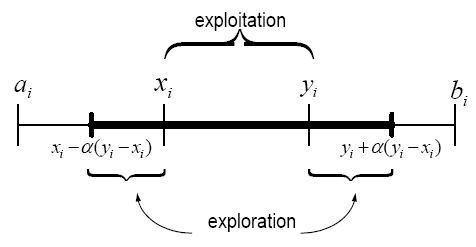
\includegraphics[width=5cm]{fig/blxalpha.jpg}
		\caption{Blend crossover operator (BLX-$\alpha$)}
		\label{fig:blxalpha}	
	\end{center}	
\end{figure}

Thus, this operator is based on the random generation of genes from the associated neighborhood of the genes in the parents. Three generated descendants are different among them and also among them and their parents, leading to a higher exploration factor in the generation of the offspring.
This operator is suitable for real coded genetic algorithms and it has proved to achieve a good balance between exploration and exploitation \cite{blx2008}.

In the Blend crossover operator, the $\alpha$ parameter values can control the exploration/exploitation rate. So, in order to ensure the balance between exploitation and exploration of the search space, $\alpha = 0.5$ could be selected.

In GAs, the search process needs a high exploration rate in the first generations to explore multiple parts of the search space so to obtain high diversity but in the last generations, high exploitation is preferred to ensure the optimal solution.

We have considered two different approaches in the experiments, one taking a  constant value of $\alpha$, and another with a variable scheme, in which the value of $\alpha$ is decreased over the generations (getting sequentially more exploitation and less exploration). Thus, its value is obtained applying the following expression:

\begin{equation}
\label{eqalpha}
\alpha =1-\frac{g}{g_{max}}
\end{equation}

Where $g$ is the current generation and $g_{max}$ is the maximum number pf generations. We think that this approach can achieve an effective balance between exploitation and exploration and therefore, better solutions may be reached.



%%%%%%%%%%%%%%%%%%%%%%%%%%  NEW RIVAL  %%%%%%%%%%%%%%%%%%%%%%%%%%%%

%\section{A New Opponent}  
%\label{sec:new-opponent}

% >>>>>> TODO: Describe "S&PL Controller" -> Antonio  <<<<<<<<<<

 


%%%%%%%%%%%%%%%%%%%%%%%%%%%%  RESULTS  %%%%%%%%%%%%%%%%%%%%%%%%%%%%

\section{Experiments and results}  
\label{sec:results}

% >>>>>> TODO: Explain the new experiments and results -> Mohammed  <<<<<<<<<<
% TODO: Results with Race-based selection (no BLX-Alpha crossover)
% TODO: Results with Race-Based selection and BLX-Alpha crossover
% TODO: Comparison against the standard controllers in TORCS
% TODO: Comparison against S&PL controller (of all our controllers, if possible)

On the basis of the results of our previous paper \cite{salem_cig2018}, the selection of an appropriate track for training is an important factor in order to obtain competitive bots. To this end we have selected for the experiments the \textbf{Alpine 2} circuit. It is a quite complex one, with multiple turns, but also straight parts (See Figure \ref{fig:alpine2_track}).

\begin{figure}[!ht]	
  \begin{center}
    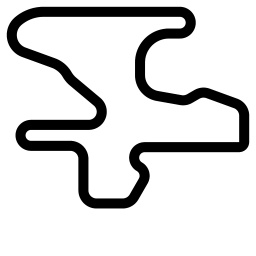
\includegraphics[width=3cm]{fig/alpine2.jpg}
    \caption{Alpine 2 Track: Slow mountain road. Length: 3773.57m, Width: 10m}
    \label{fig:alpine2_track}	
  \end{center}	
\end{figure}

As in our others studies, we have used the vehicle \textit{car1-tbr1} for our controllers, since it has a moderate performance, which will lead our controller to be prepared to drive in the most usual conditions.

We have evaluated the Genetic Fuzzy Controller (GFC) with the proposed fitness function: $AVG$ (Equation \ref{fit2}). We have run the algorithm with a population size of 60 individuals. The rest of parameters are: Generations=50, Crossover rate=0.85, Mutation rate=0.09, and 10 different runs per configuration.

New pole position selection was carried out where 10 races are used to compete every 10 individuals/controllers of the population.
We used 5 races (of 5 laps) in the \textit{Alpine 2} track (used in the optimization) and 5 races (of 5 laps) in \textit{E-Track 5} track (a new one for them). 
In order to enhance the selection of the best, another two controllers are picked randomly from the default TORCS bots to participate in the race. Moreover, in order to do it fairer, we have defined a \textit{score}, so the controller which gets the fastest lap or the minimum damage in each race is given 5 points.
% Antonio - Mohammed, this is the explanation of the race-based selection policy, right? If so, I'll copy this explanation (or a part of it) to the GA section. ;)
% Or is it the description of the final selection of the best?


The evolution process was applied in separate bunches of runs to obtain the following controllers:
\begin{itemize}
	\item $GFC$: Controller  from our previous work \cite{salem_cig2018} 
using race-based selection only in the final generation and with fitness  $f_{AVS}$ (Equation \ref{fit2}).
	\item $GFC-RS$: A controller obtained by applying two points
          crossover operator. Pole selection is applied once every five
          generations; fitness $f_{AVS}$ in all the others. 
	\item $GFC-FA$: A controller obtained by applying BLX-$\alpha$
          crossover operator with a constant value of $\alpha=0.5$ and
          pole selection once every 5 generations and fitness
          $f_{AVS}$ in the others. 
	\item $GFC-VA$: A controller obtained by applying BLX-$\alpha$
          crossover operator with a varying value of $\alpha$ using
          Equation \ref{eqalpha} and pole selection once every 5
          generations and fitness $f_{AVS}$ in the others. 
\end{itemize}
% Antonio - Mohammed, are you performing also a race-based selection at the end of the evolution to choose the best of all the controllers, as it was done in GFC?

% If this happens at the end, you should clarify - JJ 
These genetic fuzzy based controllers are evaluated in some practice
races together in a kind of Formula 1 {\em mini championship}, consisting of
10 races, each one for 20 laps, and with a total of 10 participants
per race: the 4 genetic fuzzy controllers and also 6 bots from TORCS
are used to test our controllers. The first 5 races are conducted in
\textit{Alpine 2} track (trained one); and the other 5 races took
place in \textit{E-Track 5} track (not trained for the new
controllers, but used in the evolution of our previous ones). 
The results are shown in Table \ref{tab:chsresults} and summarized
graphically in Figure \ref{fig:gfc_races}. 
%
\begin{table*}[ht]
  \centering
  {\scriptsize
    \caption{ Results of the mini-championship with 10 drivers and 10
      races in two different tracks. {\tt tita}, {\tt berniw} and {\tt
      inferno} are example controllers included with the TORCS
    simulator \cite{torcs4}}
    {
			\begin{tabular}{|c||c|c|c|c|c|c||c|c|c|c|c|c||c|}
				\hline
			&\multicolumn{6}{|c|}{Races in \textit{Alpine 2} track (20 laps each)} &	\multicolumn{6}{|c|}{Races in \textit{E-Track 5} track (20 laps each)}&\\
					\cline{2-13}
Driver&{R1}&{R2}&{R3}&{R4}&{R5}&Track Score&{R6}&{R7}&{R8}& {R9}&{R10}&Track Score& Total Score\\
				\hline
$GFC$	&	6&	8&	8&	15&15		&52&	12&	15&	10&	10&	15&62&134\\
$GFC-RS$&	12&	10&	18&	12&12		&64&	10&	8&	12&	25&	8&63&127\\
$GFC-FA$&	18&	12&	15&	10&10		&65&	15&	12&	25&	15&	25&92&157\\
$GFC-VA$&	25&	18&	25&	25&18		&111&	25&	18&	15&	18&18	&94&205\\
$tita1$	&	4&	2&	6&	4&1			&15&	2&	1&	2&	1&	1&7&22\\
$tita2$	&	2&	1&	2&	2&2			&9&	1&	2&	1&	2&	2&8&17\\
$inferno1$&	8&	4&	1&	1&6			&20&	4&	4&	6&	8&	6&28&48\\
$inferno2$&	1&	6&	4&	8&8			&27&	6&	6&	4&	4&	4&24&51\\
$berniw1$&	10&	25&	10&	18&4		&67&	18&	10&	8&	12&	12&60&127\\
$berniw2$&	15&	15&	12&	6&25		&73&	8&	25&	18&	6&	10&67&140\\
\hline
				
			\end{tabular}
		}\label{tab:chsresults}
	}
\end{table*}
%


\begin{figure}[!ht]	
	\begin{center}
		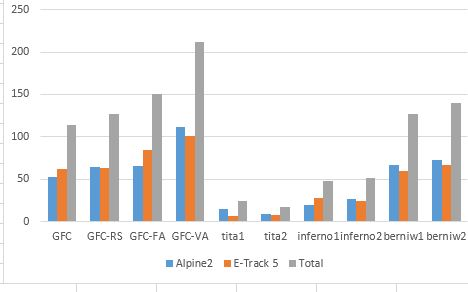
\includegraphics[width=8cm]{fig/gfc_races.jpg}
		\caption{Scores obtained by the different Genetic fuzzy-based controllers in two different tracks.}
		\label{fig:gfc_races}
                % Please don't use screen captures for figures. Also,
                % the little circles around one of the bars make no
                % sense - JJ
	\end{center}
\end{figure}
% Antonio - Mohammed, please, generate the figure without the "dots" in blue bars. Also put the correct name of the track "E-Track 5".

It is clear from the table and figure that the $GFC-VA$ controller
yields the best results in the evaluation process. Indeed, The
proposed controller won three races in Alpine 2 track and has been
ranked in the second place in the two other racing tracks. In the E-Track 5
circuit, it won two races, has been second twice and third in
the last race.

The second controller using the BLX-$\alpha$ (constant value of 0.5)
operator came second in all races. It won one race and was ranked
second in two more and third in three races.
The other races were won by the $berniw$ controller, always a tough rival.
We can notice that the BLX-$\alpha$ based controllers won three out of the five races in the Alpine 2 track used in the selection and were ranked at least in fourth place.
The same results or even  better were obtained for the other track, which is supposed to be unknown for our controllers.

These results confirm the effectiveness and strength of the pole position selection policy used to evaluate individuals as well as to select candidates for crossover. Although this policy has been applied only once every 5 generations due to its time-consuming, it has clearly affected the performance of the obtained controllers looking to the large gap between the results of the $GFC$ controller against $GFC-RS$ one.

This proposed selection policy (which also includes mutation),
combined with the BLX-$\alpha$ operator, has improved the performance
of the $GFC-FA$ controller. 
The introduction of a variable $\alpha$ parameter along the
generations in $GFC-VA$ bot has made it possible to better control the
exploration/exploitation ratio during the evolutionary process,
allowing to generate descendants different from their parents in genes
and more efficient than them. 

% -------------------------------------------

\textbf{Comparison with PSRI controller.}

In order to check the value of the obtained controller using our algorithm, we have conducted an additional experimentation.

We have considered an opponent from the state of the art, which participated in several Simulated Car Racing Competitions in past editions. 
It was proposed by P{\'e}rez-Li{\'e}bana, S{\'a}ez, Recio and Isasi \cite{EvolvingRuleSystem08} and later refined in the work \cite{PerezEvolvingFuzzy09}. We have baptised it as PSRI in honor of its authors' surnames.

This controller behaves mainly using a Finite State Machine (FSM), defining the main states in which the driver can be (for instance turning, overtaking a rival). The transitions in the FSM are governed by a set of fuzzy rules, based on the information read from different sensors. There is also a classifier module (J48 decision tree), able to analyse the inputs from some sensors in order to predict parts of the track, to anticipate the following actions to perform. The fuzzy rules and also some parameters of the FSM were optimized by means of a NSGA-II algorithm.

As stated, PSRI controller competed in 2009 edition of the Simulated
Car Racing Championship \cite{SimulatedCarRacing-2010}, where it was
ranked 4th considering the scores obtained in three different
Competitions (held at CEC, GECCO and CIG 2009 conferences). It
performed very well on average, reaching good scores and positions in
several races.

Table \ref{tab:damagespeed} presents a comparison between the two
BLX-$\alpha$ genetic based fuzzy controllers presented in this paper,
\textbf{$GFC-FA$} and \textbf{$GFC-VA$} with PSRI controller. The
results are the average values of $damage$, $MaxSpeed$ and $Speed$ of
10 races in the \textit{Alpine 2} and \textit{E-Track 5} tracks. 


\begin{table}[!ht]
  \centering
  {\scriptsize
    \caption{Average damage and Speed Results of 5 races in
      \textbf{Alpine 2} and 5 races in \textbf{E-Track 5} tracks}
    % Average should always go with standard deviation - JJ
    \label{tab:damagespeed}
    \begin{tabular}{|p{1.65cm}|c|c|c|}
      \hline 
      \multicolumn{4}{|c|}{\textbf{Alpine 2}}  \\	
      \hline  
   & \textbf{$GFC-FA$}&\textbf{$GFC-VA$} & \textbf{$PSRI$}\\					
      \hline \textbf{Average Speed (km/h)}& 187.11&199.65&176.94\\
      \hline \textbf{Max Speed (km/h)}& 225.07&231.91&217.83\\	
      \hline \textbf{Damage}& 126.82& 117.55&131.99 \\	
      \hline \textbf{Won races}&0&4&1\\	
      
      \hline 
    \end{tabular}
    \begin{tabular}{|p{1.65cm}|c|c|c|}
      \multicolumn{4}{|c|}{\textbf{E-Track 5}}  \\
      \hline 
& \textbf{$GFC-FA$}&\textbf{$GFC-VA$} & \textbf{$PSRI$}\\				
      \hline \textbf{Average Speed (km/h)}& 161.11&170.23&160.89\\
      \hline \textbf{Max Speed  (km/h)}&262.88&270.17&266.54\\	
      \hline \textbf{Damage}&18.12& 14.67&28.09\\	 
      \hline \textbf{Won races}&1&3&1\\	
      \hline 
    \end{tabular}
	}
\end{table} 

The results of the $PSRI$ controller and $GFC-FA$ are very close, they won two and one race respectively among 10. Their average speeds are similar but as for the damage, the controller $GFC-FA$ suffered the minimum because of the inclusion of the variable $damage$ in the fitness evaluation.
The results of the $GFC-VA$ controller are very satisfactory. Indeed, it won 7 races and got the lowest value of damage $117.55$ and $14.67$ for both circuits, the highest average speed $199.65$ and $170.23$.

Looking at these and previous results, we can conclude that the proposed controllers are very successful, due to the new included mechanisms to deal with uncertainty and to perform a more convenient search of the space of solutions.



%%%%%%%%%%%%%%%%%%%%%%%%%%%%  CONCLUSIONS  %%%%%%%%%%%%%%%%%%%%%%%%%%%%
\section{Conclusions and Future Work} 
\label{sec:conclusions}

% >>>>>> TODO: Rewrite this section -> All  <<<<<<<<<<


These results let us to think that our controller could have reached a very good rank in the Simulated Car Racing Competition, which is unfortunately over since 2013. Anyway, we think that the findings of this study (and previous ones) could be applied successfully to other car racing simulators, such as those used in current eSports Competitions, such as iRace (https://www.iracing.com/).



\section*{Acknowledgments}

This work has been supported in part by: Ministerio espa\~{n}ol de
Econom\'{\i}a y Competitividad under projects  TIN2017-85727-C4-2-P (UGR-DeepBio) and TEC2015-68752 (also funded by FEDER).

\bibliographystyle{IEEEtranS}
\bibliography{fuzzy_torcs}

\end{document}
